\documentclass[12pt]{article}
\usepackage[utf8]{inputenc}
\usepackage[french]{babel}
\usepackage[tikz]{bclogo}
\usepackage{geometry}
\usepackage{array}
\usepackage{version}
\usepackage{graphics}
\usepackage{graphicx}
\usepackage{url}
\usepackage{enumitem}
\bibliographystyle{alpha}
\usepackage[counterclockwise]{rotating}
\geometry{hmargin=2.5cm,vmargin=1.5cm}

\setlength{\parskip}{1ex plus 2ex minus 1ex}
\newcolumntype{M}[1]{
    >{\raggedright}m{#1}
}
\setlist[description]{topsep=20pt}

\title{
 \begin{minipage}\linewidth
        \centering
        Partitionnement de graphe 
        \vskip3pt
        \large Rapport de projet
    \end{minipage}
 }
 
\bibliographystyle{alpha}
\author{Kévin Barreau \and Guillaume Marques}

\begin{document}

\maketitle

\abstract
L'objectif du projet est d'implémenter différentes méthodes de partitionnement de graphe, vu précédemment en cours, afin des les comparer. Il s'agit de méthode exhaustive, avec l'énumération, d'algorithme glouton, avec la descente de gradient, et de métaheuristiques, avec le recuit simulé, la recherche Tabou et l'algorithme génétique. Le langage de programmation pour atteindre ce but est libre (Javascript a été choisi pour ce projet). Les résultats sont présentés de deux façons : une comparaison des résultats obtenus par les différentes méthodes sur les mêmes instances de graphe, ainsi qu'une visualisation en temps réel de la meilleure solution trouvée par les méthodes.

\newpage

\renewcommand{\contentsname}{Sommaire} 
\tableofcontents

\newpage

\section{Présentation du projet}

\subsection{Description du problème}

\paragraph{}À partir d'un graphe non orienté, il faut partitionner le graphe en K classes au moyen de plusieurs métaheuristiques, de telle sorte que la somme des poids entre sommets n'appartenant pas à la même classe soit minimale. De plus il faut s'assurer que les sommets du graphe soient répartis de manière (à
peu prés) équitable. C'est un problème NP-complet.
\paragraph{}Nous avons choisi d'utiliser comme notion d'équité une représentation par un seuil de tolérance dans la différence entre la taille du plus grand cluster et la taille du plus petit cluster. Par exemple, pour un graphe de 10 sommets, un partitionnement en 3 classes avec une tolérance de 2 autorise une solution de la forme $\mathbf{\left\langle 2,4,4 \right\rangle}$ ($4-2 = 2$, inférieur ou égal à la tolérance) mais n'autorise pas une solution de la forme $\mathbf{\left\langle 2,3,5 \right\rangle}$ ($5-2 = 3$, strictement supérieur à la tolérance).
\paragraph{}Le nombre de classe et la tolérance sont paramétrables.

\subsection{Méthodes de résolution}

\paragraph{}Pour résoudre ce problème, nous avons implémenté plusieurs algorithmes.
\begin{itemize}
	\item Énumération
	\item Descente de gradient
	\item Recuit simulé
	\item Méthode Tabou
	\item Algorithme génétique
\end{itemize}

\paragraph{}L'énumération est une méthode exhaustive, qui parcours toutes les solutions possibles pour garder le meilleur résultat. La solution finale est la solution optimale du problème.

\paragraph{}La descente de gradient est un algorithme glouton, qui, à partir du voisinage d'une solution, se déplace vers le meilleur résultat améliorant. On ne revient donc jamais sur une solution déjà visitée. La solution finale n'est pas forcément la solution optimale du problème.

\paragraph{}Le recuit simulé, la méthode Tabou et l'algorithme génétique sont des métaheuristiques, cherchant une solution en essayant de ne pas avoir le plus gros problème de la descente de gradient : rester bloquer dans un optimum local. La solution finale n'est pas forcément la solution optimale du problème.

\subsection{Choix de mise en œuvre}

\paragraph{}Pour implémenter les différentes méthodes de partitionnement de graphe, nous avons choisi d'utiliser le langage de programmation Javascript. Ce dernier apporte de nombreux avantages comme :
\begin{itemize}
	\item Rapidité d'écriture (langage interprété à typage dynamique)
	\item Accessibilité (un navigateur web suffit pour l'exécution)
	\item Visualisation (HTML, CSS, Canvas, WebGL...)
\end{itemize}

\paragraph{}On peut cependant lui reprocher une lenteur relative, comparé à des langages comme C++ ou Java. Dans un problème d'optimisation comme celui du partitionnement de graphe, on cherche toujours les meilleures performances possibles. Cependant, nous avons voulu abordé ce projet comme une introduction aux différentes méthodes et à leur comparaison, et non comme une implémentation la plus optimisée qui soit.

\paragraph{}Les structures de données utilisées sont ainsi orientées vers le besoin d'affichage des résultats, non vers le besoin de performance. Les performances de mémoire sont principalement impactées, car plusieurs représentation du graphe sont utilisées (liste de sommets et d'arêtes pour la visualisation, matrice d'adjacence pour les algorithmes).

\paragraph{}Ce choix de langage nous permet aussi d'apporter une interface graphique riche à moindre coût. Toutes les méthodes sont ainsi paramétrables par le biais de cette interface, sans avoir besoin de modifier et de recompiler le code.

\section{Implémentation des méthodes de partitionnement de graphes}

\paragraph{}Chaque méthode possède sa propre façon de fonctionner. Il faut donc être capable de réaliser des opérations identiques sur des codages de solutions différents, qui correspondent à la structure de données pour enregistrer une solution. Nous avons utilisé 2 codages : une \textbf{liste de partitions} et un \textbf{tableau}.
\paragraph{}Les méthodes de partitionnement de graphes utilisent aussi des fonctions de voisinage. Le voisinage correspond aux solutions atteignables à partir d'une solution, en faisant un mouvement élémentaire. Nous avons choisi d'implémenter 2 mouvements élémentaires : le \textbf{swap} et le \textbf{pick'n'drop fallback swap}.

\subsection{Codage des solutions}

\subsubsection{Liste de partitions}

\paragraph{}La liste de partitions est un tableau de tableau. Le premier tableau correspond aux classes, chaque case représentant une classe pour le partitionnement du graphe. L'index dans ce tableau correspond au numéro de la classe. Chaque case est composée d'un tableau. Ce deuxième tableau possède le numéro des sommets appartenant à la classe. L'index dans ce tableau ne correspond à rien contrairement au précédent tableau.

\paragraph{}Prenons comme exemple un graphe de 5 sommets partitionné en 2 classes, avec les sommets 0 et 3 dans la classe 0, et les sommets 1, 2 et 4 dans la classe 1. On obtient alors la solution sous la forme $\mathbf{[[0,3],[1,2,4]]}$.

\subsubsection{Tableau unique}

\paragraph{}Le tableau unique correspond,comme son nom l'indique, à un simple tableau. Sa taille est égale au nombre de sommets dans le graphe, et chaque index du tableau correspond au numéro d'un sommet. La valeur de chaque case est le numéro de classe auquel appartient le sommet ayant pour index cette case.

\paragraph{}Prenons comme exemple un graphe de 5 sommets partitionné en 2 classes, avec les sommets 0 et 3 dans la classe 0, et les sommets 1, 2 et 4 dans la classe 1. On obtient alors la solution sous la forme $\mathbf{[0,1,1,0,1]}$.

\subsection{Méthodes de voisinage}

\subsubsection{Swap}

\paragraph{}Le mouvement de swap consiste, à partir d'une solution, à échanger de place deux éléments de cette solution. Dans le cas du partitionnement de graphe, ce mouvement est réalisé en prenant un premier sommet dans une classe, un deuxième sommet dans une autre classe, et en les échangeant de classe.

\paragraph{}Un exemple de swap avec un graphe de 5 sommets partitionné en 2 classes, avec les sommets 0 et 3 dans la classe 0, et les sommets 1, 2 et 4 dans la classe 1 serait :
\begin{enumerate}
	\item Dans la classe 0, prendre le sommet 3
	\item Dans la classe 1, prendre le sommet 1
	\item Mettre le sommet 3 dans la classe 1
	\item Mettre le sommet 1 dans la classe 0
\end{enumerate}
On passe donc d'une solution $\mathbf{[0,1,1,0,1]}$ à une solution $\mathbf{[0,0,1,1,1]}$.

\paragraph{}Le swap est un mouvement qui \textbf{conserve la structure} de la solution de départ. C'est à dire que si la solution possède 3 classes avec 5 sommets dans chacune des classes, le mouvement ne modifiera pas cette configuration. Dans le cas où la tolérance ne dépasse pas 1, ce n'est pas un problème car il n'y a qu'une configuration possible. Mais si la tolérance est supérieure à 1, le mouvement de swap ne permettra pas d'atteindre toutes les solutions possibles du problème.

\paragraph{}La taille du voisinage avec le mouvement swap est égale à
\begin{large}$\sum\limits_{i=1}^{p-1} \sum\limits_{j=i+1}^p k_i k_j$\end{large}, avec $k_i$ le nombre de sommets dans la classe $i$. Si l'on prend $k=\frac{n}{p}$, on retrouve une estimation de l'ordre de $n^2$.

\paragraph{}Afin de gagner du temps, nous évaluons la nouvelle solution à partir de la précédente solution et du mouvement effectué. Il n'est pas nécessaire de tout recalculer, mais de seulement calculer la variation engendrée par le mouvement. Pour la méthode du swap, il suffit, pour les 2 sommets échangés, d'ajouter à l'évaluation précédente le poids des arêtes entre eux et leur ancienne classe, et de soustraire le poids des arêtes entre eux et leur nouvelle classe.

\subsubsection{Pick'n'drop fallback swap}

\paragraph{}Le mouvement de pick'n'drop consiste, à partir d'une solution, à déplacer un élément de cette solution. Dans le cas du partitionnement de graphe, ce mouvement est réalisé en prenant un sommet dans une classe et en le déplaçant dans une autre classe.

\paragraph{}Un exemple de pick'n'drop avec un graphe de 5 sommets partitionné en 2 classes, avec les sommets 0 et 3 dans la classe 0, et les sommets 1, 2 et 4 dans la classe 1 serait :
\begin{enumerate}
	\item Dans la classe 0, prendre le sommet 3
	\item Mettre le sommet 3 dans la classe 1
\end{enumerate}
On passe donc d'une solution $\mathbf{[0,1,1,0,1]}$ à une solution $\mathbf{[0,1,1,1,1]}$.

\paragraph{}Comme on peut le voir dans l'exemple, le pick'n'drop est un mouvement qui \textbf{ne conserve pas la structure} de la solution de départ. Une solution de départ $\mathbf{\left\langle 5,5,5 \right\rangle}$ aura ainsi une configuration différente après ce mouvement de type $\mathbf{\left\langle 4,5,6 \right\rangle}$. Cela implique que la tolérance peut ne plus être respectée suite à un pick'n'drop (une tolérance de 1 dans cette exemple ne permet pas de réaliser ce mouvement).
\paragraph{}C'est pourquoi nous avons ajouté un système de \textbf{fallback}, qui consiste à réaliser un un deuxième pick'n'drop si la contrainte de tolérance n'est pas respectée. Si l'on reprend l'exemple précédent, on obtient une nouvelle solution 
$\mathbf{[0,1,1,1,1]}$, qui ne satisfait pas une tolérance de 1. On réalise alors un pick'n'drop en prenant un sommet dans la classe dans laquelle nous avons ajouté un nouvel élément, et en le mettant dans l'ancienne classe de cet élément. On retombe alors sur un mouvement de \textbf{swap}. En choisissant le sommet 1, on obtient la solution $\mathbf{[0,0,1,1,1]}$, ce qui revient à avoir fait le même mouvement que dans l'exemple du swap.

\paragraph{}La taille du voisinage avec le mouvement pick'n'drop est égale à
\begin{large}$n\left(p-1\right)$\end{large}, avec $n$ le nombre de sommets dans le graphe et $p$ le nombre de classe. Si l'on ajoute le voisinage atteignable par le fallback, on obtient alors une taille de voisinage pour ce mouvement compris entre la taille du voisinage de pick'n'drop et la taille du voisinage de swap, dépendant de la tolérance et du nombre de sommet du graphe par rapport au nombre de classe.

\paragraph{}Afin de gagner du temps, nous évaluons la nouvelle solution à partir de la précédente solution et du mouvement effectué. Il n'est pas nécessaire de tout recalculer, mais de seulement calculer la variation engendrée par le mouvement. Pour la méthode du pick'n'drop, il suffit, pour le sommet déplacé, d'ajouter à l'évaluation précédente le poids des arêtes entre lui et son ancienne classe, et de soustraire le poids des arêtes entre lui et sa nouvelle classe. Si on retombe sur le fallback swap, il suffit de réaliser l'évaluation partielle de la méthode swap.

\subsection{Méthodes de résolution}

\subsubsection{Énumération}

\paragraph{}La méthode énumérative consiste à parcourir toutes les solutions possibles du problème. C'est à dire que pour un graphe à $n$ sommets que l'on cherche à partitionner en $k$ classes, il existe $k^n$ solutions possibles. Ce nombre augmente ainsi exponentiellement avec la taille du problème, ce qui rend cette méthode utilisable seulement sur de très petites instances de graphe.

\paragraph{}Pour énumérer toutes les solutions, nous avons utilisé une technique de sac à dos, en nous inspirant de l'implémentation Python de Marc-Michel Corsini pour résoudre ce problème. Le principe de cette technique est de faire évoluer une solution afin de parcourir toutes les configurations possibles, à partir d'un codage de solution de type tableau.

\paragraph{}On commence à partir d'une solution vide, et on ajoute le premier sommet dans la première classe et on passe au sommet suivant. Lorsque qu'on ajoute un sommet, on le met dans la première classe qui n'est pas pleine (principe de "quasi-équilibre" des classes). S'il n'y a pas de classe disponible, on revient au sommet précédent et on le met dans la première classe disponible supérieure à sa classe actuelle. On a trouvé une solution quand le nombre de sommet dans la solution est égale au nombre de sommets du graphe. L'algorithme s'arrête lorsque la solution est vide.

\paragraph{}Cette technique réalise un parcours exhaustif. Cependant, on peut réaliser certaines coupes lorsque une solution partielle ne respecte pas la contrainte de tolérance. Il n'est alors pas nécessaire de voir les solutions suivantes, car elles posséderont aussi cette solution partielle qui n'est pas valide. Une autre coupe consiste à ne pas regarder certaines solutions symétriques. En effet, une solution $\mathbf{[0,0,1,1,1]}$ et $\mathbf{[1,1,0,0,0]}$ sont équivalentes étant donné que la numéro d'une classe n'a pas d'importance. Pour éviter ce type de solution, le numéro de classe maximum, pour chaque sommet d'index $i$, est égale à $\min\left(i,k-1\right)$. Ainsi, le premier sommet ne peut être que dans la classe 0, le deuxième dans la classe 0 ou 1, etc. On divise ainsi le nombre de solutions parcourues par $k$ sans perdre l'exhaustivité (nous avons supprimé seulement des symétries).

\paragraph{}Pour comprendre l'algorithme, faisons le tourner sur un exemple simple : un graphe à 4 sommets en 2 classes.

\begin{table}[h]
\centering
\begin{tabular}{|l|c|}
	\hline
	solution & valide ? \\
	\hline
	$\mathbf{[0]}$ & non \\
	$\mathbf{[0,0]}$ & non \\
	$\mathbf{[0,0,1]}$ & non \\
	$\mathbf{[0,0,1,1]}$ & oui \\
	$\mathbf{[0,0,1]}$ & non \\
	$\mathbf{[0,1]}$ & non \\
	$\mathbf{[0,1,0]}$ & non \\
	$\mathbf{[0,1,0,1]}$ & oui \\
	$\mathbf{[0,1,1]}$ & non \\
	$\mathbf{[0,1,1,0]}$ & oui \\
	$\mathbf{[0,1,1]}$ & non \\
	$\mathbf{[0,1]}$ & non \\
	$\mathbf{[0]}$ & non \\
	$\mathbf{[]}$ & non \\
	\hline
\end{tabular}
\end{table}

\paragraph{}On obtient ainsi 3 solutions valides, que l'on évalue et dont on garde la plus petite valeur d'évaluation.

\subsubsection{Descente de gradient}

\paragraph{}La descente de gradient est un algorithme consistant à trouver un optimum local.
Il ne s'agit donc pas de la solution optimale mais d'une des meilleures solution.

\paragraph{}Nous choisissons une solution initiale que nous définissons comme \textbf{solution courante}. Nous cherchons dans son voisinage, une meilleure solution.
S'il y en a une, nous la définissons comme \textbf{solution courante}, puis répétons l'opération.
S'il n'y en a pas, nous avons trouvé la solution optimale locale et l'algorithme est terminé.
Nous remarquons que la solution finale trouvée dépend de la solution initiale choisie.


\paragraph{}Dans cette implémentation, nous cherchons dans le voisinage de la \textbf{solution courante}, la meilleure solution parmi les solutions meilleures que la \textbf{solution courante} et non une meilleure solution.
L'avantage est que la résolution se fait en moins d'itérations mais l'inconvénient est que la recherche prend plus de temps. En effet, nous devons parcourir tout le voisinage.
Dans certains cas, il faut donc préferer la deuxième méthode. 
Nous convergeons vers l'optimum local en plus d'itérations mais le fait de ne pas parcourir la totalité du voisinage à chaque itération peut-être un gain de temps non négligeable.
Travaillant sur des petits graphes, nous avons choisi la première méthode.

\subsubsection{Recherche Tabou}

\paragraph{}La recherche Tabou est une amélioration de l'algorithme de la descente de gradient. Il ne s'arrête pas lorsqu'il trouve un optimum local.
Son fonctionnement est le même mais dans une file, nous stockons les $n$ derniers mouvements utilisés pour trouver les $n$ dernières \textbf{solutions courantes}.

\paragraph{}A chaque itération, nous cherchons dans le voisinage de la \textbf{solution courante}, la meilleure solution possible.
Nous stockons dans la file le mouvement $m$ nous ayant permis de trouver cette solution.

\paragraph{Exemple Pick'n'drop} Considérons une solution obtenue en déplacant le noeud $2$ de la partition $A$ vers la partition $B$, le mouvement est donc $<A,B,2>$.

\paragraph{Exemple Swap} Considérons une solution obtenue en échangeant le noeud $2$ de la partition $A$ et le noeud $3$ de la partition $C$, le mouvement est donc $<A,C,2,3>$.

\paragraph{}Dans la prochaine recherche d'une meilleure solution dans le voisinage, le mouvement $m^{-1}$ sera interdit.
En effet, cela permet de ne pas revisiter une solution.
Si la solution précédente était l'optimum local, l'algorithme de la recherche tabou ne restera pas bloqué sur l'optimum local et pourra donc en chercher un autre.


\paragraph{}La taille de la file est limitée pour éviter une perte de performance lors de la recherche des mouvements interdits (il faut parcourir toute la file pour s'assurer qu'un mouvement n'est pas dedans).
L'ordre des mouvements n'ayant pas d'importance et afin de limiter le nombre d'opérations (maj de la file) nous utilisons un tableau circulaire.

\paragraph{Exemple} Dans une tableau de taille $k$, le $m$ième mouvement utilisé sera stocké en position $m\%k$. Nous conservons bien les $k$ derniers mouvements.


\subsubsection{Recuit simulé}

\paragraph{}Le recuit simulé est un algorithme stochastique inspiré de la thermodynamique. Son principe repose sur une première phase de refroidissement rapide, qui va tendre à augmenter la phase d'exploration de l'algorithme. Au fur et à mesure du temps, la température baisse de moins en moins vite et l'on se retrouve dans une situation de descente de gradient, correspondant à une phase d'exploitation. Ce changement de phase progressif est rendu possible grâce à l'\textbf{algorithme de Metropolis} qui modélise une chaîne de Markov à distribution stationnaire.

\paragraph{}Le recuit simulé est considéré comme une méta-heuristique du fait de ses nombreux paramètres indéterminés, inhérents au problème que l'on cherche à résoudre. Pour le problème de partitionnement de graphe, nous avons décidé d'implémenter une grande partie de ces paramètres, et de les rendre modifiables à partir d'une interface graphique.

\paragraph{}La \textbf{solution initiale} est le point d'entrée de l'algorithme, la solution sur laquelle on commence à travailler. Elle est très importante, car bien choisie, elle permet d'accélérer le processus vers la recherche de la meilleure solution. Mais attention, même avec une solution qui parait bonne de prime abord, il est possible de se retrouver avec l'effet inverse de celui escompté car cette solution peut se retrouver loin (en terme de voisinage) de la solution optimale. Pour le projet, nous avons tout d'abord utilisé comme solution initiale la première solution valide de la méthode énumérative. Cependant la solution est assez mauvaise, et toujours identique. Nous avons alors décidé d'utiliser un \textbf{générateur de solution aléatoire}. Les solutions du générateur sont toutes "quasi-équilibrée", ne prenant pas en compte la tolérance. De possibles améliorations seraient donc de prendre en compte la tolérance, ou alors de générer une solution en sortie d'un algorithme glouton (pour obtenir une première solution pas trop mauvaise).

\paragraph{}La \textbf{température initiale}, en adéquation avec le \textbf{facteur de refroidissement}, détermine les phases d'exploration et d'exploitation de l'algorithme. La température évolue au cours du temps suivant une suite géométrique de raison $q$, $q$ étant le facteur de refroidissement. Refroidir trop vite et la phase d'exploration sera très courte, revenant à faire une descente de gradient. Refroidir trop lentement et la phase d'exploration sera très longue, entraînant une augmentation importante du temps de traitement ou une faible phase d'exploitation suivant les conditions d'arrêt. Nous avons décidé de mettre ces 2 paramètres en \textbf{paramètres d'initialisation} de l'algorithme, c'est à dire que nous ne faisons aucun traitement dessus, ils doivent être défini à la main. Nous avons cependant remarqué, de manière empirique, qu'une température entre 20 et 50 avec un facteur de refroidissement entre 0.85 et 0.95 donnait des résultats satisfaisants, offrant un bon compromis entre le temps d'exécution et la valeur de la solution finale.

\paragraph{}La \textbf{condition d'arrêt} de l'algorithme peut être défini de nombreuses manières. Nous avons décidé d'en implémenter la plupart afin de laisser le choix de la méthode à la configuration. Parmi ces méthodes, nous avons :
\begin{itemize}
\item un \textbf{nombre fixe d'itérations}, que nous la faisons généralement osciller entre 100 et 200.
\item une \textbf{température de gel}. L'algorithme s'arrête quand la température courante est inférieure à celle de gel.
\item un \textbf{seuil de stabilité} de la solution, qui correspond au nombre d'itérations maximale sans que la meilleure solution ne change.
\end{itemize}

\paragraph{}Le seuil de stabilité est très efficace pour les graphes de petites instances, tandis qu'on préférera travailler avec la température de gel ou le nombre fixe d'itérations pour les plus gros graphes.

\paragraph{}La \textbf{condition de bouclage interne} est une boucle permettant de trouver la meilleure solution à température constante. C'est cette boucle qui itère sur l'algorithme de Metropolis. Il faut avoir un nombre d'itération suffisant afin d'avoir la propriété de stabilité des chaînes de Markov. Pour la condition d'arrêt de cette boucle, nous avons opté pour une suite géométrique avec les paramètres du \textbf{nombre d'itérations (metropolis)} et du \textbf{facteur d'itération (metropolis)}. On peut ainsi choisir entre un nombre  d'itération constant avec une raison de 1, ou augmenter/diminuer le nombre d'itération suivant le temps pour agir sur la durée des phases d'exploration et d'exploitation. Dans la plupart de nos tests, un nombre d'itération de l'ordre de 50 suffisait. Mais ce paramètre tend à augmenter proportionnellement à la taille du graphe.

\paragraph{}Le \textbf{voisinage} est la méthode permettant de passer d'une solution à une autre. L'algorithme du recuit simulé choisit une solution aléatoirement dans le voisinage de la solution actuelle. Il est possible d'utiliser le \textbf{swap} ou le \textbf{pick'n'drop}, avec les avantages et inconvénients que cela implique comme nous l'avons présenté dans la section concernée.

\subsubsection{Algorithme génétique}

\paragraph{}Quelques paramètres. Mutation swap ou pick'n'drop. Croisement de 2 manières différentes. Sélection par roulette, système de mating pool. Meilleure solution reste d'une génération à l'autre. Codage de solution tableau (passage liste pour mutation).

\paragraph{}Les algorithmes génétique sont inspirés de la biologie, avec les principes de sélection naturelle et de génétique. Ils consistent à faire évoluer une population de génération en génération, se basant sur la survie des éléments les plus résistants pour qu'ils se reproduisent et créent les futures générations. On converge alors petit à petit vers une solution optimale.

\paragraph{}Pour le problème de partitionnement, un \textbf{individu} correspond à une solution à notre problème. Les solutions seront sous la forme d'un codage type tableau. Chaque case du tableau représente un \textbf{gène}. A chaque génération, on répète le même processus qui est : évaluation, sélection, croisement, mutation. Le nombre de génération et le nombre d'individu dans une population sont paramétrables à partir de l'interface graphique.

\paragraph{}La première étape du processus, l'\textbf{évaluation}, consiste à calculer la \textbf{fitness} de chaque individu de la population. Nous avons choisi d'utiliser comme fonction de fitness : $\forall_{i \in population}, fitness(i) = v_{max} - v_i + 1$ avec $v_i$ la valeur de la solution $i$ et $v_{max}$ la plus grande valeur de solution dans la population. On obtient ainsi une fitness où les meilleurs solutions possèdent une plus grande valeur, et la moins bonne solution est égale à 1. Cette transformation va nous être utile pour l'étape de sélection.

\paragraph{}La deuxième étape du processus est l'étape de \textbf{sélection}, dans laquelle on va prendre des individus de la population au hasard avec plus ou moins de chance d'être pris suivant leur fitness. Pour cette étape, nous avons opté pour l'utilisation d'une \textbf{mating pool} (que l'on peut traduire par \textit{piscine d'accouplement}). Nous parcourons chaque individu de la population actuelle, et nous mettons autant de fois l'individu dans la mating pool que la partie entière de $100\frac{fitness_i}{fitness_{total}}$. Avec la partie résiduelle, notée $pr$ (les chiffres après la virgule), on réalise un tirage aléatoire entre 0 et 1, noté $p$, et si $p < pr$ alors on ajoute encore une fois l'individu à la mating pool. Cela permet de garder de la constance dans les choix si jamais on se retrouve avec une valeur de 1.01 et une autre de 0.98. Les deux valeurs sont proches ont doivent avoir à peu près la même chance d'être sélectionné. On obtient alors une mating pool remplie grâce à notre population.

\paragraph{}La troisième étape est celle du \textbf{croisement}. Il s'agit de créer de nouveaux individus à partir de ceux déjà existants, en échangeant des portions de gènes. Pour choisir les individus parents, on pioche aléatoirement dans la mating pool créée précédemment. On a alors une probabilité d'avoir un croisement entre deux individus piochés, probabilité définie en paramètre. Nous avons choisi de faire un \textbf{croisement à deux points}, c'est à dire que l'on prend deux points au hasard et que l'on échange la portion située entre les deux points. Cependant, cette technique n'assure pas une solution valide après le croisement. C'est pourquoi nous avons réfléchi à deux méthodes d'équilibrage.
\paragraph{}La première consiste à remplacer la portion comme un remplissage sac à dos. On essaie de mettre la nouvelle portion gène par gène. Si un gène n'était pas présent dans l'ancienne portion, on ne le met pas. On remplit ensuite les trous avec les gènes manquants de l'ancienne portion. Cette méthode a l'avantage de créer des solutions valides, mais ne tire pas parti de toutes les spécificités du croisement (on n'a pas vraiment échangé les portions).
\paragraph{}La seconde méthode réalise un échange pur et dur. Cependant, si la solution n'est pas valide, on pénalise sa valeur suivant le degré de violation de la contrainte de tolérance. Cela permet de garder des solutions peut-être non valide, mais qui possède des portions de gènes intéressantes pour de futurs croisements. Il est par contre compliqué de trouver une bonne fonction de pénalisation permettant de garder ces solutions à leur juste valeur.

\paragraph{}La dernière étape est la \textbf{mutation}. Elle permet d'explorer un peu plus l'espace de recherche en s'appliquant aléatoirement sur les gènes. Pour des raisons de performances, il n'est pas intéressant de réaliser un jet de dé pour savoir si on réalise une mutation pour chaque gène de chaque individu de la population. Nous avons donc décidé de mettre un nombre de mutation par génération en paramètre, qui s'appliqueront sur un individu au hasard. Les mutations sont des \textbf{mouvements élémentaires}, donc dans notre cas un swap ou un pick'n'drop.

\section{Résultats}

\section{Présentation du code}

\subsection{Diagramme de classe (général)}

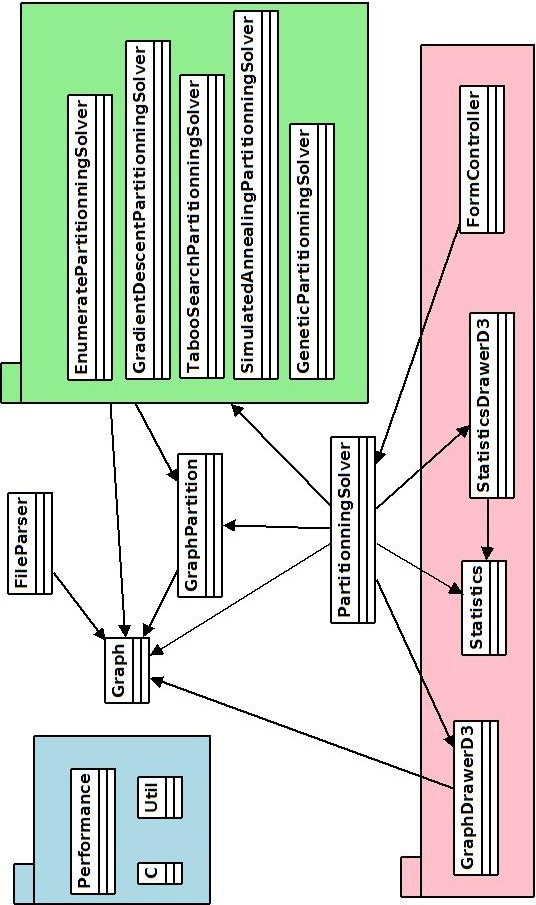
\includegraphics[height=20cm]{classeGraph.jpeg}

\subsection{Explications}

\paragraph{}On peut découper le code en plusieurs grandes familles de classes, visibles en partie dans le diagramme de classes.

\paragraph{}La première famille, en rouge dans le diagramme de classe, correspond aux classes ayant un rapport avec l'\textbf{interface graphique}. La classe \textit{FormController} est la porte d'entrée de l'application. Elle s'occupe des événements provenant du formulaire de paramètre. Il y a ensuite les classes préposées aux graphiques, avec \textit{GraphDrawerD3} pour le graphe, prenant les données de la classe \textit{Graph}, et \textit{StatisticsDrawerD3} pour les statistiques, prenant les données de la classe \textit{Statistics}.

\paragraph{}La deuxième famille est la plaque tournante de l'application, avec la classe \textit{PartitionningSolver} et sa méthode \textit{resolve} qui récupère les paramètres pour la résolution du problème, initialise tout ce qui est nécessaire et lance la résolution. On peut lui adjoindre la classe \textit{Graph}, qui est la représentation du graphe à résoudre en mémoire, ainsi que la classe \textit{GraphPartition} qui s'occupe des traitements sur les partitions : voisinages, évaluations, codages.

\paragraph{}La troisième famille, en vert dans le diagramme de classe, est celle des \textbf{méthodes de résolution}. On y retrouve les 5 méthodes implémentées (énumération, descente de gradient, recuit simulé, recherche tabou et algorithme génétique), chacune d'elle ayant sa propre classe. Elles reposent sur la même architecture (l'héritage n'existe pas en Javascript) avec comme point d'entrée une méthode \textit{resolve}.

\paragraph{}La dernière famille correspond aux \textbf{classes d'aide} pour les différentes tâches à faire. Ainsi, la classe \textit{Performance} permet de chronométré précisément la durée d'une fonction, la classe \textit{C} s'occupe de la sortie sur console, la classe \textit{Util} regroupe des fonctions de nécessité générale par rapport au langage en lui-même (copie d'objet, génération d'entier aléatoirement...), et la classe \textit{FileParser} lit les fichiers de graphes pour les créer dans la classe \textit{Graph}.

\end{document}
